\documentclass[11pt]{article}

\usepackage[margin=1in]{geometry}
\usepackage{amsmath}
\usepackage{booktabs}
\usepackage{graphicx}
\usepackage[hidelinks]{hyperref}
\usepackage{pgfplots}
\pgfplotsset{compat=1.18}

\title{DMRG Cylinder Benchmarks and Charge Pump Notes}
\author{Partial Hall Crystal Project}
\date{\today}

\newcommand{\phitwopi}{\Phi_y/2\pi}
\newcommand{\qmid}{Q_{\mathrm{mid}}}

\begin{document}
\maketitle

\section{Purpose}

This document is a living LaTeX notebook for the DMRG branch. It collects benchmark
numbers, production run parameters, charge-pump figures, and short interpretation
notes. Generated DMRG outputs are intentionally kept outside git; only summary
numbers and lightweight plots should be recorded here.

\section{Model and Geometry}

The DMRG module studies the full two-band real-space model on a cylinder. The
geometry is open along \(x\) and periodic along \(y\). For the Ly=6 cylinders used
below,
\[
  N_s = L_x L_y, \qquad N_{\mathrm{uc}} = N_s/2 = 3L_x,
  \qquad N_p = N_{\mathrm{uc}}/3 = L_x .
\]
The production parameter set is
\[
  t_1=1.0,\qquad t_3=0.2,\qquad V_1=1.0,\qquad V_2=V_3=0.0 .
\]

\section{Cylinder ED vs DMRG Benchmark}

The first small-system verification compared DMRG against exact diagonalization
of the same cylinder Hamiltonian, not against the torus Hamiltonian. The data are
stored on W003 in
\begin{center}
\small\path{dmrg/output_Lx4/energy_check.dat}.
\end{center}

\begin{table}[h]
\centering
\caption{Lx=4, Ly=6, Np=4 cylinder benchmark at zero flux.}
\begin{tabular}{llr}
\toprule
Quantity & Method & Energy \\
\midrule
Ground-state energy & cylinder ED & \(-9.238777471721946\) \\
Ground-state energy & DMRG & \(-9.238777009200746\) \\
Absolute difference & \(|E_{\mathrm{DMRG}}-E_{\mathrm{ED}}|\) & \(4.6252120000644936\times 10^{-7}\) \\
\bottomrule
\end{tabular}
\end{table}

The torus ED result for the tracked 4x6, Np=4 data set is instead
\[
  E_{\mathrm{torus}} \simeq -9.31357589 .
\]
Thus
\[
  E_{\mathrm{cyl}} - E_{\mathrm{torus}}
  \simeq 0.07479842 .
\]
This is a boundary-condition effect: the cylinder drops hopping and interaction
terms that cross the open \(x\) boundary and has physical edges. The ED--DMRG
agreement above validates the cylinder MPO and sign/index conventions; it does
not imply equality to the torus spectrum.

\section{Lx=15 Production Run}

The main charge-pump production run used
\[
  L_x=15,\quad L_y=6,\quad N_s=90,\quad N_{\mathrm{uc}}=45,\quad
  N_p=15,\quad \nu=N_p/N_{\mathrm{uc}}=1/3 .
\]

\begin{table}[h]
\centering
\caption{Production DMRG settings for the Lx=15 charge pump.}
\begin{tabular}{ll}
\toprule
Item & Value \\
\midrule
Campaign directory & \texttt{dmrg/flux\_Lx15\_pump\_prod\_20260710\_170505} \\
Flux direction & \(y\)-cycle twist on the cylinder \\
Max bond dimensions & \(200,400,800,1200,1600,2000\) \\
Cutoff & \(10^{-9}\) \\
Energy tolerance & \(10^{-6}\) \\
Density tolerance & \(2\times10^{-5}\) \\
Truncation-error tolerance & \(5\times10^{-8}\) \\
Threading target & 24 CPU cores per node on W003 \\
\bottomrule
\end{tabular}
\end{table}

\section{Charge Pump Observable}

The plotted charge is the cumulative density change to the left of a middle
cut:
\[
  Q(x,\Phi_y)=\sum_{x'\le x,y}
  \left[\langle n_{x',y}\rangle_{\Phi_y}
  - \langle n_{x',y}\rangle_{\Phi_y=0}\right].
\]
The plotted quantity is \(\qmid\), evaluated near the center of the cylinder.
The total right-edge cumulative charge is approximately zero because the total
particle number is fixed.

\section{Flux Insertion Result}

The charge-pump plot data were generated from
\begin{center}
\small\path{/home/public/shajy/partial_Hall_crystal/dmrg/flux_Lx15_pump_prod_20260710_170505/plots/charge_pump_plot_data.csv}.
\end{center}
The plotted campaign contains 48 converged points from three trajectories:
\begin{itemize}
  \item \path{forward_pi12}
  \item \path{branch_from_fwd17_pi24}
  \item \path{branch_from_fwd17_pi36}
\end{itemize}

\begin{table}[h]
\centering
\caption{Selected points from the forward \(\Delta\Phi=\pi/12\) trajectory.}
\begin{tabular}{rrrr}
\toprule
\(\phitwopi\) & Step & Raw \(\qmid\) & Unwrapped \(\qmid\) \\
\midrule
0.000000 & 0  & 0.000000000 & 0.000000000 \\
0.250000 & 6  & 0.082319845 & 0.082319845 \\
0.500000 & 12 & 0.166481976 & 0.166481976 \\
0.750000 & 18 & 0.254744645 & 0.254744645 \\
0.791667 & 19 & 0.269989638 & 0.269989638 \\
0.833333 & 20 & -0.054694482 & 0.278638851 \\
1.000000 & 24 & -0.000000131 & 0.333333202 \\
\bottomrule
\end{tabular}
\end{table}

\begin{figure}[p]
\centering
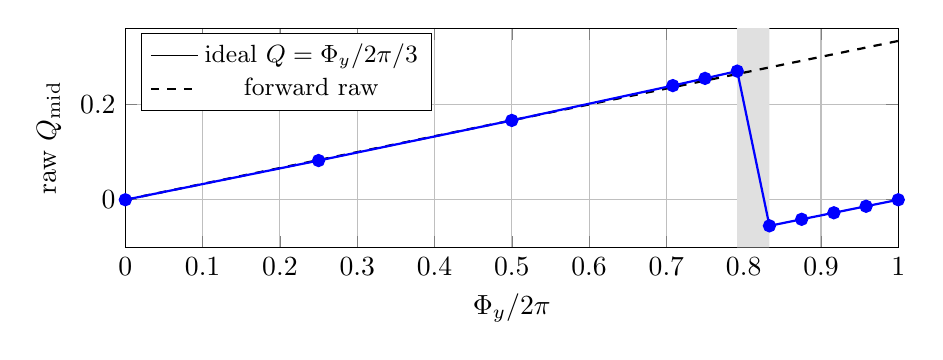
\begin{tikzpicture}
\begin{axis}[
    width=0.94\linewidth,
    height=0.36\linewidth,
    xmin=0, xmax=1,
    ymin=-0.10, ymax=0.36,
    xlabel={\(\phitwopi\)},
    ylabel={raw \(\qmid\)},
    grid=both,
    legend style={at={(0.02,0.98)},anchor=north west,font=\small},
]
\addplot[draw=none,fill=black!12] coordinates {
  (0.791667,-0.10) (0.833333,-0.10) (0.833333,0.36) (0.791667,0.36)
} \closedcycle;
\addplot[dashed,thick] coordinates {(0,0) (1,0.333333333)};
\addlegendentry{ideal \(Q=\phitwopi/3\)}
\addplot[blue,thick,mark=*] coordinates {
  (0,0)
  (0.25,0.082319845)
  (0.5,0.166481976)
  (0.708333,0.239594793)
  (0.75,0.254744645)
  (0.791667,0.269989638)
  (0.833333,-0.054694482)
  (0.875,-0.040987639)
  (0.916667,-0.027309661)
  (0.958333,-0.013650770)
  (1.0,-0.000000131)
};
\addlegendentry{forward raw}
\end{axis}
\end{tikzpicture}

\vspace{0.8cm}

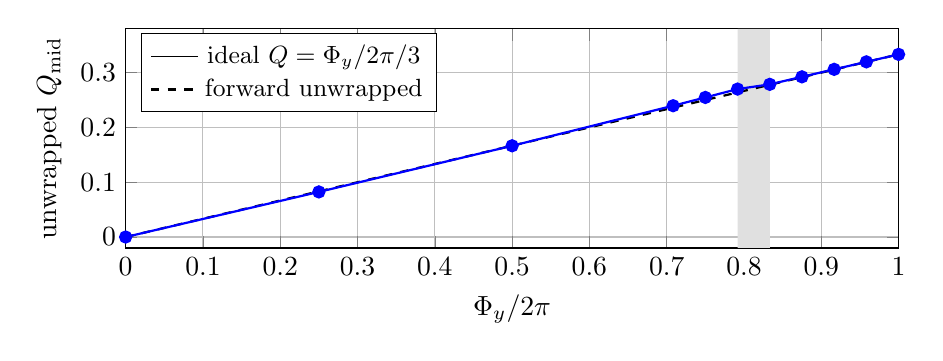
\begin{tikzpicture}
\begin{axis}[
    width=0.94\linewidth,
    height=0.36\linewidth,
    xmin=0, xmax=1,
    ymin=-0.02, ymax=0.38,
    xlabel={\(\phitwopi\)},
    ylabel={unwrapped \(\qmid\)},
    grid=both,
    legend style={at={(0.02,0.98)},anchor=north west,font=\small},
]
\addplot[draw=none,fill=black!12] coordinates {
  (0.791667,-0.02) (0.833333,-0.02) (0.833333,0.38) (0.791667,0.38)
} \closedcycle;
\addplot[dashed,thick] coordinates {(0,0) (1,0.333333333)};
\addlegendentry{ideal \(Q=\phitwopi/3\)}
\addplot[blue,thick,mark=*] coordinates {
  (0,0)
  (0.25,0.082319845)
  (0.5,0.166481976)
  (0.708333,0.239594793)
  (0.75,0.254744645)
  (0.791667,0.269989638)
  (0.833333,0.278638851)
  (0.875,0.292345695)
  (0.916667,0.306023672)
  (0.958333,0.319682564)
  (1.0,0.333333202)
};
\addlegendentry{forward unwrapped}
\end{axis}
\end{tikzpicture}
\caption{Summary charge-pump curves. The gray band marks the branch-switch window
\(0.791667 \le \phitwopi \le 0.833333\). The lower panel unwraps the
post-switch sector by adding \(1/3\) to the raw charge.}
\label{fig:charge-pump-summary}
\end{figure}

\section{Branch-Switch Interpretation}

The raw charge jumps from about \(0.270\) to about \(-0.055\), a change close to
\(-1/3\). The unwrapped curve assumes this is a topological-sector switch and
adds \(1/3\) after the jump:
\[
  Q_{\mathrm{unwrapped}} =
  \begin{cases}
    Q_{\mathrm{raw}} + 1/3, & \phitwopi > 0.78 \ \mathrm{and}\ Q_{\mathrm{raw}}<0.08,\\
    Q_{\mathrm{raw}}, & \mathrm{otherwise}.
  \end{cases}
\]
This produces \(Q_{\mathrm{unwrapped}}(2\pi)\simeq 0.3333332\), consistent with
one-third charge pumping. This is a useful summary plot, but the branch
assignment should eventually be supported by overlap tracking or entanglement
spectrum flow.

\section{Open Checks}

\begin{itemize}
  \item Add a systematic cylinder ED benchmark table for \(L_x=2,3,4\) and several flux points.
  \item Compare density profiles between cylinder ED and DMRG for the same small systems.
  \item Add branch tracking diagnostics: MPS overlaps, entanglement spectrum flow, and sector labels.
  \item Extend the pump figure to \(6\pi\) when a full three-sector cycle is available.
\end{itemize}

\end{document}
